\subsection{Числа сочетаний. Треугольник Паскаля. Рекуррентное соотношение для чисел сочетаний}

Сочетанием из $n$ по $k$ называется набор из $k$ элементов, выбранных из $n$-элементного множества, в котором не учитывается порядок элементов.
Количество сочетаний из $n$ по $k$ записывается так: $\binom{n}{k}$ или так $C^k_n$. $C^k_n =\binom{n}{k} = \frac{n!}{k!\cdot(n-k)!}$.\\ $\binom{n}{k} = \binom{n}{n-k}$.\\ $\binom{n}{k} = \binom{n-1}{k} + \binom{n-1}{k-1}$
Треугольником Паскаля называется бесконечная треугольная таблица, в которой на вершине и по боковым сторонам стоят единицы, каждое из остальных чисел равно сумме двух чисел, стоящих над ним в предшествующей строке. В таком треугольнике элемент в строке $n$ на позиции $k$ равен $\binom{n}{k}$.

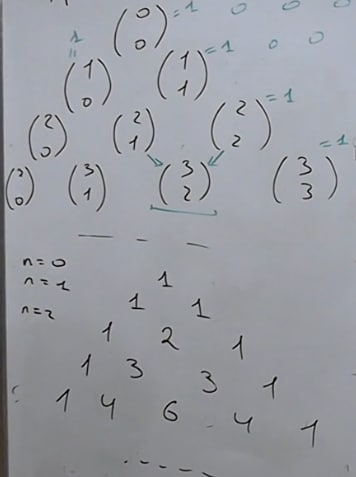
\includegraphics[scale=1]{definitions/images/pascal.png}